\documentclass[a4paper]{article}
\usepackage[a4paper,margin=0mm]{geometry}
\usepackage{fontspec}
\usepackage{unicode-math}
\usepackage{tikz}
\usepackage[table]{xcolor}
\usepackage[absolute]{textpos}
\usepackage{enumitem}
\usepackage{array}
\usepackage{multirow}

\setmainfont{Libertinus Serif}
\setsansfont{Libertinus Sans}
\setmathfont{Libertinus Math}
\newfontfamily\trackedsans{Libertinus Sans}[LetterSpace=8.0]

\definecolor{accent}{HTML}{F46530}
\definecolor{badge}{HTML}{FFBDA5}
\definecolor{ink}{HTML}{2A2E30}

\setlength{\TPHorizModule}{1mm}
\setlength{\TPVertModule}{1mm}
\setlength{\parindent}{0pt}
\pagestyle{empty}

\newcommand{\LCOL}{16mm}
\newcommand{\RCOL}{111mm}
\newcommand{\COLW}{83mm}

\newcommand{\topicheader}[2]{%
\begin{textblock*}{194mm}(16mm,10mm)
\begin{tikzpicture}
\node[fill=accent,text=white,font=\sffamily\bfseries\fontsize{13}{13}\selectfont,
      minimum width=9mm,minimum height=9mm,inner sep=0pt] at (4.5mm,-4.5mm) {#1};
\node[font=\sffamily\bfseries\fontsize{15}{16}\selectfont,text=ink,anchor=west] at (12mm,-4.5mm) {#2};
\end{tikzpicture}
\end{textblock*}
\begin{textblock*}{194mm}(16mm,22.5mm)

\begin{tikzpicture}
\fill[accent] (0,0) rectangle (194mm,0.5mm);
\end{tikzpicture}
\end{textblock*}
}

\newcommand{\pagefooter}[1]{%
\begin{textblock*}{194mm}(8mm,286.41mm)
  
\begin{tikzpicture}
    \fill[accent] (0,0) rectangle (194mm,0.6mm);
  \end{tikzpicture}
\end{textblock*}
\begin{textblock*}{63.59mm}(8mm,288.27mm)
  {\sffamily\bfseries\color{accent}\fontsize{13}{16}\selectfont SAT 1200+}
\end{textblock*}
\begin{textblock*}{10mm}(188mm,288.27mm)
  \centering{\sffamily\color{accent}\fontsize{14}{16}\selectfont #1}
\end{textblock*}
}

\newcommand{\colrule}[2]{%
\begin{textblock*}{1mm}(105mm,#1mm)
\begin{tikzpicture}
\draw[black!65,line width=0.5pt] (0,0) -- (0,#2mm);
\end{tikzpicture}
\end{textblock*}
}

\newcommand{\setkicker}[2]{%
{\sffamily\bfseries\fontsize{12}{14}\selectfont #1.}\ {\itshape\fontsize{11}{14}\selectfont\color{black!75} #2}\par\vspace{2mm}%
}

\setlength{\fboxsep}{1.4pt}
\setlength{\fboxrule}{0.5pt}
\newcommand{\pnum}[1]{\fcolorbox{ink}{white}{\sffamily\bfseries\fontsize{8}{8}\selectfont #1}~}

\newcommand{\qrbox}[1]{%
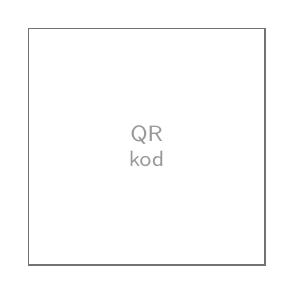
\begin{tikzpicture}
\draw[black!55,line width=0.6pt] (0,0) rectangle (30mm,30mm);
\node[black!40,font=\sffamily\fontsize{8}{9}\selectfont,align=center] at (15mm,15mm) {QR\\kod};
\end{tikzpicture}\\[1.5mm]
{\sffamily\fontsize{9}{11}\selectfont\color{black!70} #1}%
}

\arrayrulecolor{accent}
\setlength{\arrayrulewidth}{0.7pt}
\renewcommand{\arraystretch}{1.35}
\newcommand{\anstitle}[1]{{\sffamily\bfseries\color{accent}\fontsize{11}{13}\selectfont #1}\\[1.3mm]}

\begin{document}

% ================= PAGE 1: Set 1 | Set 2 =================
\topicheader{14}{Foizlar va kontekstli masalalar}
\pagefooter{1}
\colrule{32}{238}
\mbox{}%

\begin{textblock*}{\COLW}(\LCOL,32mm)
{\fontsize{11}{14}\selectfont
\setkicker{1-to'plam}{Foiz o'zgarishini toping. O'sish yoki kamayish ekanini ayting.}

\noindent\pnum{1} Narx \$40 dan \$52 ga ko'tarildi.\\[14mm]
\noindent\pnum{2} Aholi soni $2{,}500$ dan $2{,}125$ ga kamaydi.\\[14mm]
\noindent\pnum{3} Test bahosi $60$ dan $75$ ga ko'tarildi.\\[14mm]
\noindent\pnum{4} Oylik ijara \$800 dan \$880 ga ko'tarildi.\\[14mm]
\noindent\pnum{5} Aksiya narxi \$120 dan \$90 ga tushdi.\\[14mm]
\noindent\pnum{6} Son $45$ dan $54$ ga ko'tarildi.
}
\end{textblock*}

\begin{textblock*}{\COLW}(\RCOL,32mm)
{\fontsize{11}{14}\selectfont
\setkicker{2-to'plam}{Yangi qiymatni toping. Ko'paytuvchi usulidan ($\times(1{+}r)$ yoki $\times(1{-}r)$) foydalaning, ayirib-qo'shish usulidan emas.}

\noindent\pnum{1} \$250 ni $12\%$ ga oshiring.\\[14mm]
\noindent\pnum{2} \$360 ni $25\%$ ga kamaytiring.\\[14mm]
\noindent\pnum{3} $80$ ni $35\%$ ga oshiring.\\[14mm]
\noindent\pnum{4} $500$ ni $8\%$ ga kamaytiring.\\[14mm]
\noindent\pnum{5} $150$ ni $60\%$ ga oshiring.\\[14mm]
\noindent\pnum{6} $720$ ni $45\%$ ga kamaytiring.
}
\end{textblock*}

\clearpage

% ================= PAGE 2: Set 3 | Set 4 =================
\topicheader{14}{Foizlar va kontekstli masalalar}
\pagefooter{2}
\colrule{32}{238}
\mbox{}%

\begin{textblock*}{\COLW}(\LCOL,32mm)
{\fontsize{10.5}{13.5}\selectfont
\setkicker{3-to'plam}{Yakuniy qiymatni va boshlang'ichdan sof foiz o'zgarishini toping.}

\noindent\pnum{1} \$200 $10\%$ ga oshdi, so'ng $10\%$ ga kamaydi.\\[13mm]
\noindent\pnum{2} \$400 $25\%$ ga oshdi, so'ng $25\%$ ga kamaydi.\\[13mm]
\noindent\pnum{3} $150$ $20\%$ ga kamaydi, so'ng $20\%$ ga oshdi.\\[13mm]
\noindent\pnum{4} \$600 $50\%$ ga oshdi, so'ng $50\%$ ga kamaydi.\\[13mm]
\noindent\pnum{5} $1{,}000$ $10\%$ ga kamaydi, so'ng $10\%$ ga oshdi.\\[13mm]
\noindent\pnum{6} $240$ $30\%$ ga oshdi, so'ng $30\%$ ga kamaydi.
}
\end{textblock*}

\begin{textblock*}{\COLW}(\RCOL,32mm)
{\fontsize{10.5}{13.5}\selectfont
\setkicker{4-to'plam}{Yakuniy qiymat va sof foiz o'zgarishini toping.}

\noindent\pnum{1} \$300 $20\%$ oshdi, so'ng $10\%$ oshdi.\\[13mm]
\noindent\pnum{2} \$500 $20\%$ oshdi, so'ng $10\%$ kamaydi.\\[13mm]
\noindent\pnum{3} \$800 $25\%$ kamaydi, so'ng $20\%$ oshdi.\\[13mm]
\noindent\pnum{4} \$150 $40\%$ oshdi, so'ng $30\%$ kamaydi.\\[13mm]
\noindent\pnum{5} \$400 $15\%$ kamaydi, so'ng $25\%$ oshdi.\\[13mm]
\noindent\pnum{6} \$600 ketma-ket ikki marta $15\%$ ga oshdi (bitta $30\%$ bilan adashtirmang).
}
\end{textblock*}

\clearpage

% ================= PAGE 3: Set 5 (word problems) | Set 6 (spot the error) =================
\topicheader{14}{Foizlar va kontekstli masalalar}
\pagefooter{3}
\colrule{32}{238}
\mbox{}%

\begin{textblock*}{\COLW}(\LCOL,32mm)
{\fontsize{10}{13}\selectfont
\setkicker{5-to'plam}{Aralash matnli masalalar.}

\noindent\pnum{1} \$120 lik kurtka $25\%$ chegirma bilan sotiladi, so'ng chegirmali narxga $8\%$ soliq qo'shiladi. Yakuniy narxni toping.\\[9mm]
\noindent\pnum{2} $10{,}000$ kishilik shahar aholisi 1-yilda $8\%$ o'sadi, 2-yilda $5\%$ kamayadi. 2 yildan keyingi sonni toping.\\[9mm]
\noindent\pnum{3} \$2{,}000 oylik maosh bir yilda $10\%$ oshadi, keyingi yili $10\%$ kamayadi. Yangi maosh va sof foiz o'zgarishini toping.\\[9mm]
\noindent\pnum{4} \$50 lik tovar chakanada $40\%$ ga qimmatlashadi, keyin chegirmada $30\%$ ga arzonlashadi. Sotuv narxini toping.\\[9mm]
\noindent\pnum{5} \$5{,}000 omonat har yili $4\%$ foiz oladi (ikkinchi yil foizi birinchi yildagi yangi balansga hisoblanadi). 2 yildan keyingi balansni toping.\\[9mm]
\noindent\pnum{6} Kompaniya daromadi inqirozda $30\%$ kamayadi, keyingi yili $30\%$ o'sadi. Boshlang'ichdan sof foiz o'zgarishini toping va nega $0\%$ emasligini bir gapda tushuntiring.
}
\end{textblock*}

\begin{textblock*}{\COLW}(\RCOL,32mm)
{\fontsize{10.5}{13.5}\selectfont
\setkicker{6-to'plam}{Xatoni toping -- qo'shish/ayirish usulidan foydalanilgan, ko'paytuvchi usulidan emas.}

\noindent\pnum{1} \textit{``Narx $30\%$ oshadi, so'ng $20\%$ tushadi. Sof o'zgarish $30\%-20\%=10\%$ o'sish.''}\\[1mm]
\hspace*{7mm}Xato va to'g'ri javob: \makebox[48mm]{\dotfill}\\[8mm]

\noindent\pnum{2} \textit{``\$200 lik tovar $50\%$ qimmatlashadi, so'ng $50\%$ arzonlashadi, demak \$200 ga qaytadi.''}\\[1mm]
\hspace*{7mm}Xato va to'g'ri javob: \makebox[48mm]{\dotfill}\\[8mm]

\noindent\pnum{3} \textit{``Talabalar soni $10\%$, keyin yana $15\%$ o'sadi, jami o'sish $10\%+15\%=25\%$.''}\\[1mm]
\hspace*{7mm}Xato va to'g'ri javob: \makebox[48mm]{\dotfill}\\[8mm]

\noindent\pnum{4} \textit{``Aksiya $40\%$ tushadi, so'ng $40\%$ ko'tariladi, demak boshlang'ich qiymatga qaytadi.''}\\[1mm]
\hspace*{7mm}Xato va to'g'ri javob: \makebox[48mm]{\dotfill}\\[8mm]

\noindent\pnum{5} \textit{``Sonning $20\%$ ni topish uchun uni $20$ ga ko'paytirish kerak.''}\\[1mm]
\hspace*{7mm}Xato va to'g'ri javob: \makebox[48mm]{\dotfill}
}
\end{textblock*}

\clearpage

% ================= PAGE 4: Set 7 (bonus) -- own page =================
\topicheader{14}{Foizlar va kontekstli masalalar}
\pagefooter{4}
\colrule{32}{238}
\mbox{}%

\begin{textblock*}{\COLW}(\LCOL,32mm)
{\fontsize{11}{14}\selectfont
\setkicker{7-to'plam}{Bonus / qiyin.}

\noindent\pnum{1} Narx $10\%$ oshadi, yana $10\%$ oshadi, so'ng $20\%$ tushadi. Sof foiz o'zgarishini toping.\\[20mm]
\noindent\pnum{2} $20\%$ chegirmadan keyin ko'ylak \$64 turadi. Dastlabki narxni toping.\\[20mm]
\noindent\pnum{3} Ikki yillik $10\%$ o'sishdan keyin shahar aholisi $12{,}100$ kishi. Boshlang'ich sonni toping.\\[20mm]
\noindent\pnum{4} Narx $r\%$ ga oshadi, so'ng xuddi shu $r\%$ ga kamayadi va boshlang'ichdan $4\%$ pastroq bo'ladi. $r$ ni toping.\\[20mm]
\noindent\pnum{5} Ketma-ket uchta $10\%$lik o'sishdan keyin qiymat $1{,}331$ ga teng. Boshlang'ich qiymatni toping.
}
\end{textblock*}

\clearpage

% ================= PAGE 5: Javoblar =================
\topicheader{14}{Foizlar va kontekstli masalalar}
\pagefooter{5}
\mbox{}%

\begin{textblock*}{194mm}(16mm,30mm)
{\bfseries\itshape\color{accent}\fontsize{19}{21}\selectfont\centering Javoblar\par}
\end{textblock*}

\begin{textblock*}{194mm}(16mm,42mm)
{\fontsize{9}{11.3}\selectfont
\centering
\renewcommand{\arraystretch}{1.25}
\begin{tabular}{|>{\centering\arraybackslash}p{24mm}|>{\centering\arraybackslash}p{9mm}|>{\centering\arraybackslash}p{30mm}|>{\centering\arraybackslash}p{9mm}|>{\centering\arraybackslash}p{30mm}|}
\hline
\rowcolor{badge!55}\textbf{To'plam} & \textbf{\#} & \textbf{Javob} & \textbf{\#} & \textbf{Javob}\\
\hline
\multirow{3}{24mm}{\centering 1-to'plam} & 1 & $+30\%$ & 2 & $-15\%$\\\cline{2-5}
 & 3 & $+25\%$ & 4 & $+10\%$\\\cline{2-5}
 & 5 & $-25\%$ & 6 & $+20\%$\\\hline
\multirow{3}{24mm}{\centering 2-to'plam} & 1 & 280 & 2 & 270\\\cline{2-5}
 & 3 & 108 & 4 & 460\\\cline{2-5}
 & 5 & 240 & 6 & 396\\\hline
\multirow{3}{24mm}{\centering 3-to'plam} & 1 & 198, $-1\%$ & 2 & 375, $-6.25\%$\\\cline{2-5}
 & 3 & 144, $-4\%$ & 4 & 450, $-25\%$\\\cline{2-5}
 & 5 & 990, $-1\%$ & 6 & 218.4, $-9\%$\\\hline
\multirow{3}{24mm}{\centering 4-to'plam} & 1 & 396, $+32\%$ & 2 & 540, $+8\%$\\\cline{2-5}
 & 3 & 720, $-10\%$ & 4 & 147, $-2\%$\\\cline{2-5}
 & 5 & 425, $+6.25\%$ & 6 & 793.5, $+32.25\%$\\\hline
\multirow{3}{24mm}{\centering 7-to'plam} & 1 & $-3.2\%$ & 2 & \$80\\\cline{2-5}
 & 3 & 10{,}000 & 4 & $r=20\%$\\\cline{2-5}
 & 5 & 1{,}000 & -- & --\\\hline
\multirow{6}{24mm}{\centering 5-to'plam} & \multicolumn{4}{p{78mm}|}{1.\ \$97.20}\\\cline{2-5}
 & \multicolumn{4}{p{78mm}|}{2.\ 10{,}260}\\\cline{2-5}
 & \multicolumn{4}{p{78mm}|}{3.\ \$1{,}980, sof $-1\%$}\\\cline{2-5}
 & \multicolumn{4}{p{78mm}|}{4.\ \$49}\\\cline{2-5}
 & \multicolumn{4}{p{78mm}|}{5.\ \$5{,}408}\\\cline{2-5}
 & \multicolumn{4}{p{78mm}|}{6.\ Sof $-9\%$. Nolga teng emas, chunki $30\%$lik o'sish allaqachon kichraygan daromadga hisoblanadi.}\\\hline
\multirow{5}{24mm}{\centering 6-to'plam} & \multicolumn{4}{p{78mm}|}{1.\ Xato -- foizlarni to'g'ridan-to'g'ri ayirgan. To'g'ri: $(1.30)(0.80)=1.04$, sof $+4\%$.}\\\cline{2-5}
 & \multicolumn{4}{p{78mm}|}{2.\ Xato -- xuddi shunday qo'shish xatosi. To'g'ri: $(1.50)(0.50)=0.75$, sof $-25\%$.}\\\cline{2-5}
 & \multicolumn{4}{p{78mm}|}{3.\ Xato -- foizlarni qo'shgan, ko'paytirish kerak edi. To'g'ri: $(1.10)(1.15)=1.265$, sof $+26.5\%$.}\\\cline{2-5}
 & \multicolumn{4}{p{78mm}|}{4.\ Xato -- teng foiz o'sish/kamayish bir-birini yo'qotadi deb o'ylagan. To'g'ri: $(0.60)(1.40)=0.84$, sof $-16\%$.}\\\cline{2-5}
 & \multicolumn{4}{p{78mm}|}{5.\ Xato -- foizni o'nlik kasrga aylantirmagan. To'g'ri: $20$ ga emas, $0.20$ ga ko'paytirish kerak.}\\\hline
\end{tabular}
}
\end{textblock*}

\begin{textblock*}{194mm}(16mm,252mm)
\centering
{\sffamily\fontsize{9.5}{11.5}\selectfont\color{black!70} Video yechimlar va qo'shimcha testlar uchun quyidagi QR kodlarni skanerlang:}\\[4mm]
\begin{minipage}[t]{32mm}\centering\qrbox{YouTube}\end{minipage}%
\hspace{16mm}%
\begin{minipage}[t]{32mm}\centering\qrbox{Telegram}\end{minipage}
\end{textblock*}

\end{document}
